\chapter{Introducci\'on}\label{cap.introduccion}
\hspace{1 cm}Cada vez es m\'as com\'un el uso de drones para labores que pueden ser muy diversas, como puede ser grabar un plano para una pel\'icula o mantener vigilado un lugar sobrevolando estas zonas. Una parte en la que se dan grandes avances es la rob\'otica a\'erea, y una parte funcionalidad concreta es la navegaci\'on aut\'onoma de \'estos, conseguir que realicen ciertas tareas sin que haya nadie controlando su ruta. Para ello hay que contar con los distintos sensores que se le pueden añadir a un drone y la forma de utilizar \'estos en beneficio propio para conseguir dicha navegaci\'on.

\hspace{1cm} En los siguientes p\'arrafos se va a realizar una breve introducci\'on sobre estos aparatos, la historia que tienen, los distintos usos que hay para ellos actualmente, su hardware y software disponible para ellos. Tambi\'en se describir\'an varios proyectos de RoboticsLab-URJC que forman parte del contexto cercano de este Trabajo de Fin de Grado.

\section{Historia de los drones}

\hspace{1cm} Los drones son conocidos como UAV (veh\'iculos a\'ereos no tripulados). El primer registro de UAV fue un globo aerost\'atico en un entorno militar en el año 1849, que se pod\'ia utilizar para sobrevolar una zona y lanzar bombas desde cierta altura sin necesidad de que hubiera ninguna persona en \'este y, por tanto, sin arriesgar una vida. Este UAV es muy distinto a lo que vino despues, principalmente porque el motor de \'este se trata de una bolsa que tiene un gas m\'as ligero que el aire, lo que le permite coger altura y jugar con las corrientes de viento para desplazarse en una direcci\'on o en otra.

\hspace{1 cm} Ya en la primera guerra mundial se comenzaron a utilizar para sobrevolar las \'areas enemigas y hacer fotos para as\'i tener un control de sus movimientos (el introducir una c\'amara en un UAV es algo que se hizo desde los primeros momentos). Estos veh\'iculos eran aviones tripulados por radiofrecuencia, por lo que se dio un gran salto con respecto al anterior, pues era mucho m\'as f\'acil su control, por lo que pod\'ian manejar su trayectoria con mucha m\'as facilidad. 

\hspace{1cm} Tambi\'en durante la primera guerra, pero m\'as desarrollado para la segunda guerra mundial, se le dio uso a \'estos para utilizarlos como explosivos, ya que pod\'ian seguir su trayectoria en todo momento y asegurarse que llegaban al destino correcto. Adem\'as de poder seguir a otros veh\'iculos en movimiento del bando enemigo y as\'i hacer que este no llegara a su destino. 

\hspace{1cm} Est\'a claro que en los inicios ten\'ian s\'olo fines militares y que su desarrollo era exclusivamente para ello. Tras la segunda guerra mundial, el avance sobre estos fren\'o en gran medida y se utilizaban para vigilancia a\'erea en zonas de conflictos, lo que llev\'o a mejorar el sistema de control haciendo as\'i que se pudieran manejar a una mayor distancia. 

\hspace{1 cm}Fue alrededor de 1980 cuando se vi\'o que la tecnolog\'ia y el software de los UAV eran de gran fiabilidad y se les pod\'ia asignar a estas tareas de mayor responsabilidad para no poner en riesgo la vida de los pilotos. Una vez no estaban los pilotos en la cabina del veh\'iculo se pod\'ia jugar con mayor libertad a la hora de realizar movimientos, ya que ciertos giros que los pilotos no pod\'ian realizar por ser demasiado bruscos para el cuerpo humano, ahora pod\'ian hacerlos con la brusquedad que permitiera el sistema.  

\hspace{1 cm} Ya en la d\'ecada de los 90 se da un avance muy importante, con el desarrollo del sistema GPS para el desplazamiento de estos veh\'iculos. Esto permit\'ia no depender de la radiofrecuencia, ya que con \'esta se tiene un l\'imite en distancia y no revisar los datos para ver en todo momento su situaci\'on y teledirigir la trayectoria. Con \'este sistema se traza una ruta al inicio y el UAV puede trabajar de forma aut\'onoma. 

\hspace{1cm} Cabe destacar el gran avance que ha sufrido la rob\'otica a\'erea e los \'ultimos años. En torno al año 2000 y en adelante, se ha profundizado en el uso civil de los drones y no tanto militar. Por un lado en la parte aeroespacial, cada veh\'iculo innovador mejora con creces al anterior debido a diseño, estructura o materiales, que permiten mayor velocidad y resistencia. Y por parte de la rob\'otica ocurre lo mismo, est\'a en un continuo desarrollo, y viendo el futuro que tienen los drones muchas empresas y grupos de investigaci\'on han decidido centrarse en ellos, pudiendo as\'i mejorar a diario el software de estos, lo que permite un control m\'as fluido, gracias al env\'io y procesamiento de informaci\'on, as\'i como controlar mejor en todo momento el estado que se encuentra el drone (bater\'ia, posicionamiento en los distintos ejes o velocidad). 
 


\section{Aplicaciones actuales }
\hspace{1 cm} En esta secci\'on se barre de manera breve las aplicaciones y distintos usos que se le dan hoy en d\'ia. Se ven en la sociedad en general para terminar viendo varios prototipos m\'as espec\'ificos de la rob\'otica a\'erea en los que se est\'a investigando, concretamente los que llevan a que este pueda trabajar de manera aut\'onoma. 

\subsection{Medios Audiovisuales}
\hspace{1 cm} El drone es un elemento que se ha incorporado \'ultimamente en este sector debido a la c\'amara que pueden tener. Gracias a esto permite tomar planos de ciertas zonas o fotograf\'ias que ser\'ian muy dif\'icil de obtener en condiciones normales. Tambi\'en se debe a que el precio de \'estos es asequible, por lo que se puede acceder a ellos con facilidad, y en un sector tan amplio y vistoso como es \'este, lleva a un uso cada vez m\'as com\'un.
\begin{figure}[H]
	\centering
		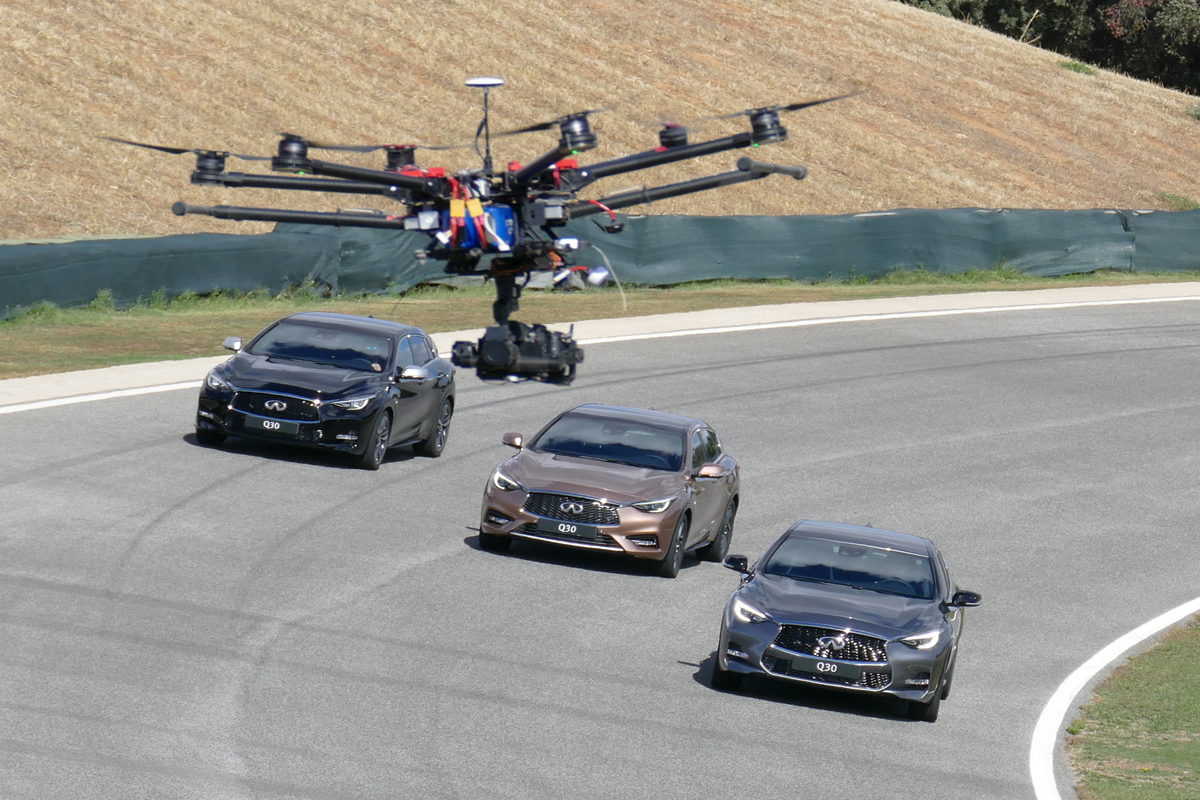
\includegraphics[width=0.4\textwidth]{imgs/anuncio_television.jpg}
				\caption{Drone grabando para la publicidad de una marca de coches.}
	\label{fig:Drone grabando publicidad.}
\end{figure}

%\subsection{Drones para el control.}
%\hspace{1 cm} En este \'area podemos destacar varios usos distintos, pero su expansi\'on en esto se debe a que con un drone podemos controlar una zona para la que anteriormente necesit\'abamos varias c\'amaras, y aun as\'i pod\'ian quedar zonas sin vigilar. \'Esta tecnolog\'ia nos lleva a poder mover una c\'amara por un lugar amplio sin necesidad de estar all\'i ni de tener un gran despliegue de elementos, as\'i como evitar que queden puntos muertos. Algunos ejemplos de esto son los siguientes: 

%\begin{itemize}
\subsection{Seguridad} 
\hspace{1 cm}Teniendo un drone en una nave industrial por ejemplo, se puede hacer que \'este se desplace grabando en todo momento lo que ve, y si se detecta algo sospechoso en alg\'un lugar el drone se dirija all\'i en el momento para obtener im\'agenes de lo que est\'a pasando. 

\begin{figure}[H]
	\centering
		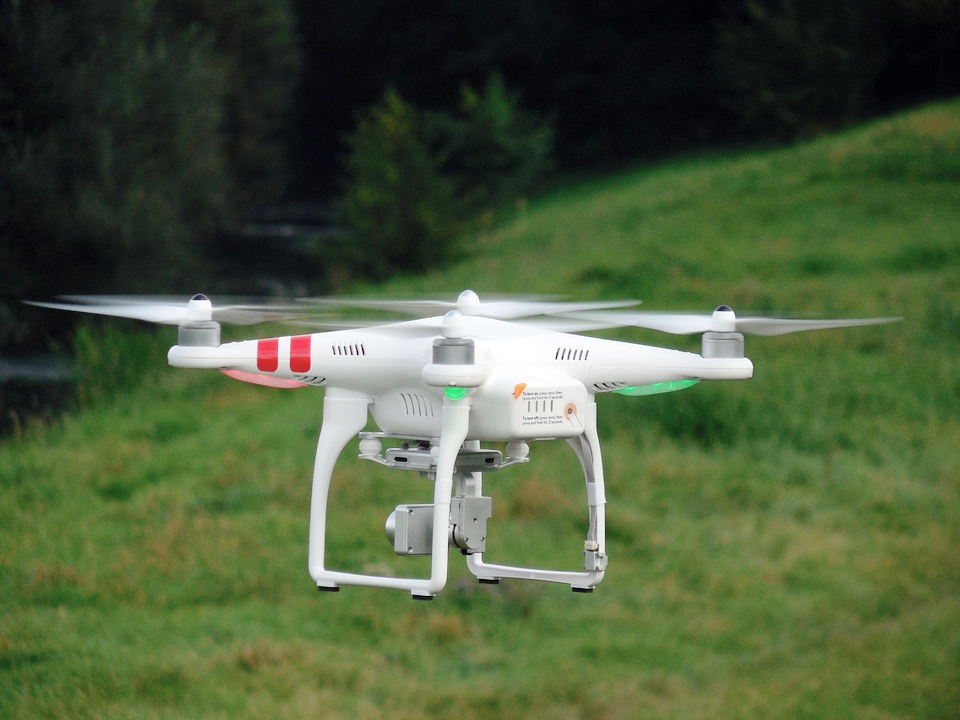
\includegraphics[width=0.25\textwidth]{imgs/seguridad_drone.jpg}
		\caption{Empresa Prevent Security Sistems utiliza drones para videovigilancia en grandes superficies .}
	\label{fig: Empresa Prevent Security Sistems realiza videovigilancia con drones.}
\end{figure}

	\subsection{Sector agr\'icola} 
\hspace{1 cm}El uso de drones en este sector se encuadra en la agricultura de precisi\'on. Se debe a la facilidad con la que un drone puede sobrevolar una zona y ofrecer im\'agenes de alta calidad, obteniendo un buena monitorizaci\'on de los cultivos en menos tiempo, con menos gasto y al tratarse de un veh\'iculo el\'ectrico al evitar desplazamientos de otros autom\'oviles conlleva un menor impacto ambiental. Adem\'as, permite ver con facilidad el estado de la cosecha, detectar enfermedades o plagas, permiten fumigar desde el aire con mayor precisi\'on, ya que les puedes programar una ruta y que sigan \'esta. Tambi\'en podr\'ian obtener otros datos como las zonas con m\'as y menos agua, y obtener las condiciones del terreno y ver si son \'optimas para esperar cierto resultado. En este tipo de drones, aparte de la c\'amara son de importancia otros sensores, como los de temperatura y humedad, o infrarrojos para captar el espectro infrarrojo de las plantas. 
	
	
\begin{figure}[H]
	\centering
		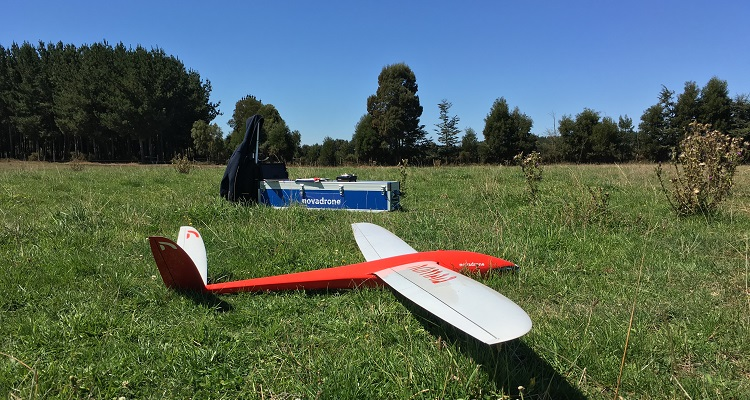
\includegraphics[width=0.4\textwidth]{imgs/novadrone.jpg}
		\caption{Empresa Novadrone utiliza drones para la gesti\'on de las explotaciones agr\'icolas .}
	\label{fig: Empresa Novadrone, aplicaciones en agricultura.}
\end{figure}

	\subsection{Inspecci\'on} 
\hspace{1 cm}En este apartado se engloban diversas actividades, como puede ser mantenimiento de edificios y construcciones, redes el\'ectricas o diversas instalaciones industriales como aerogeneradores e\'olicos y estados de paneles solares. Al igual que en el apartado anterior, aqu\'i se pueden recorrer grandes distancias, por ejemplo para comprobar las redes el\'ectricas, sin la necesidad de que un operario pierda mucho tiempo recorriendo dicha l\'inea. Con las instalaciones solares por ejemplo, desde un plano superior podr\'iamos observar si todas las placas estan en las condiciones \'optimas y en caso de existir alg\'un fallo identificarlo con facilidad. Para edificios y aerogeneradores lo que hay que tener en cuenta es la altura que pueden alcanzar, y a la cual con un drone llegar\'iamos con facilidad y observar\'iamos si hay alg\'un problema. En estos casos lo que evitamos, como anteriormente he comentado, es que alguien tenga que ir sitio a sitio perdiendo mucho tiempo. Destacando tambi\'en que este tipo de actividades se pueden implementar programas que directamente detecten las anomal\'ias, sin necesidad de que haya una persona revisando en todo momento las im\'agenes, donde tambi\'en con una inversi\'on inicial, al final ahorrar\'iamos mucho tiempo y dinero. Un ejemplo de \'esto se da en la empresa Iberdrola, la cual ha incorporado drones para el mantenimiento e inspecci\'on de sus infraestructuras, utilizando drones por ejemplo para el mantenimiento de las palas de los aerogeneradores. Uni\'on Fenosa tambi\'en ha incorporado los drones para la inspecci\'on de los tendidos el\'ectricos. 
%\end{itemize}

%\hspace{1 cm} Por otro lado, pueden aportar gran ayuda en situaciones que no se dan de forma peri\'odica, sino que ocurren de forma espor\'adica y en lugares muy distintos. Gracias a los drones podemos tener una camara que nos muestre una imagen de esta zona o que nos permita ayudar all\'i, y en otro momento llevarlo a otro lado, lo que lleva a no tener un gran despliegue de medios en un lugar que apenas va a ser necesario. Los ejemplos podr\'ian ser los siguentes:

%\begin{itemize}
	\subsection{Emergencias}
\hspace{1 cm} Cuando ocurren ciertas cat\'astrofes naturales, por ejemplo, son de gran ayuda debido a la velocidad con la que pueden llevar materiales (m\'edicos o de otro tipo) a la zona afectada. Un ejemplo de esto es el \textit{Angel Drone}, proyecto desarrollado por la universidad de Sidney, que puede llevar materiales quir\'urgicos o plasma sangu\'ineo.

\begin{figure}[H]
	\centering
		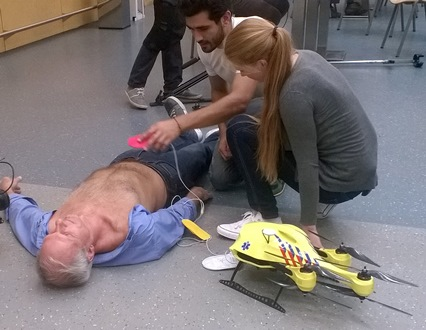
\includegraphics[width=0.4\textwidth]{imgs/drone_desfibrilador.jpg}
		\caption{Desarrollan en la universidad de Holanda un drone que lleva incorporado un desfibrilador .}
	\label{fig: Drone con desfibrilador para emergencias.}
\end{figure} 
	%\item \textbf{B\'usqueda de personas:} Al tratarse de medios que pueden sobrevolar zonas obteniendo grandes im\'agenes, pueden ser de ayuda cuando monta?eros o caminantes tienen accidentes en bosques o monta?as, quedan incomunicados y se comienza una b\'usqueda.

	%\item \textbf{Incendios forestales:} Los drones pueden estar sobrevolando zonas y obteniendo informaci\'on de esta, para as\'i poder prevenir posibles incendios o alertar lo antes posible en cuanto uno ocurra. 

%\end{itemize}

\subsection{Prototipos de investigaci\'on }
\hspace{1 cm} Determinados grupos y grandes empresas est\'an trabajando e investigando y construyendo prototipos con drones para distintas labores. Esto se debe a la facilidad que pueden ofrecer los drones para realizar tareas como el control de material en almacenes o transporte de material de un lugar a otro. Una caracter\'istica importante es la rapidez con la que pueden llegar los drones de un lugar a otro, y acceder a lugares que es dif\'icil para otros veh\'iculos. 

\hspace{1 cm} Como pionero en este \'area se encuentra \textbf{Amazon}, el cual lleva desarrollando desde 2013 una tecnolog\'ia que permita el reparto de paquetes mediante drones. La idea cuenta con doce prototipos, debido en parte a los distintos tipos de UAV que tienen.  Esta tecnolog\'ia lleva consigo los llamados almacenes a\'ereos, es decir, un almac\'en que se mantendr\'ia en el aire gracias a dirigibles, el cual tiene paquetes a entregar y drones. El drone obtendr\'ia el paquete que se debe entregar y lo llevar\'ia al lugar adecuado. Tras esto volver\'ia a un almacen hasta que se le mande de nuevo al almac\'en a\'ereo para el siguiente reparto. Estos drones sabr\'ian en todo momento en el estado y en el punto en el que se encuentran, es decir, que saben a qu\'e lugar deben ir dependiendo de la tarea a realizar. 

\begin{figure}[ht]
	\centering
		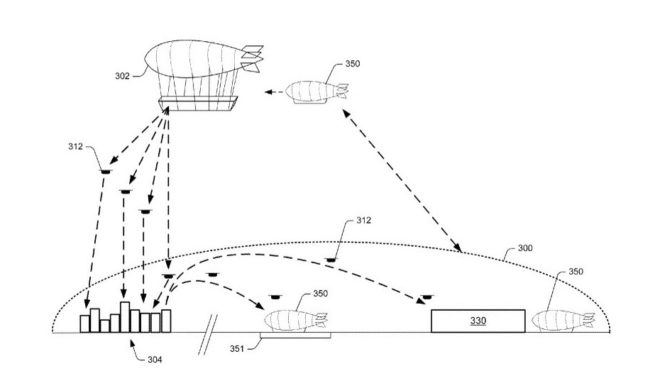
\includegraphics[width=0.55\textwidth]{imgs/amazon.jpg}
	\label{fig:Esquema de reparto con drones}
\end{figure}

\hspace{1 cm} El 7 Diciembre de 2016, Amazon Prime Air (servicio de drones repartidores) realiz\'o la primera entrega de una compra real en la regi\'on de Cambridge, Reino Unido. Se puede encontrar este video,ademas de otros, en su p\'agina web. \underline{\url{https://www.amazon.com/Amazon-Prime-Air/b?node=8037720011}}

\hspace{1 cm} Por otro lado, tambi\'en para el reparto de mercanc\'ias se encuentra \textbf{Google}, llegando a tener un programa piloto en Australia en el año 2014, pero no consigui\'o llevarlo a Estados Unidos. Aun as\'i, consigui\'o hacer pruebas de reparto de comida en una universidad, un reto que supuso principalmente que la comida llegara r\'apido a su destino y en buenas condiciones. Adem\'as, tambi\'en sirvi\'o para ajustar los sistemas autom\'aticos de vuelo y entrega de la mercanc\'ia. 

\hspace{1 cm} A ra\'iz de estos servicios de entregas se ha producido otro desarrollo importante, como puede ser el de tener controlados los paquetes dentro de un almac\'en. Un pionero de esto ha sido un grupo en el \textbf{MIT}, desarrollando un sistema que permite a los drones moverse por los almacenes escaneando los c\'odigos de cada paquete, enviando esta informaci\'on a un servidor y que \'este pueda tener controlados los paquetes que hay y d\'onde est\'an situados. 

\begin{figure}[H]
 \centering
  \subfloat[RFID detectado]{
   \label{f:RFID detectado}
    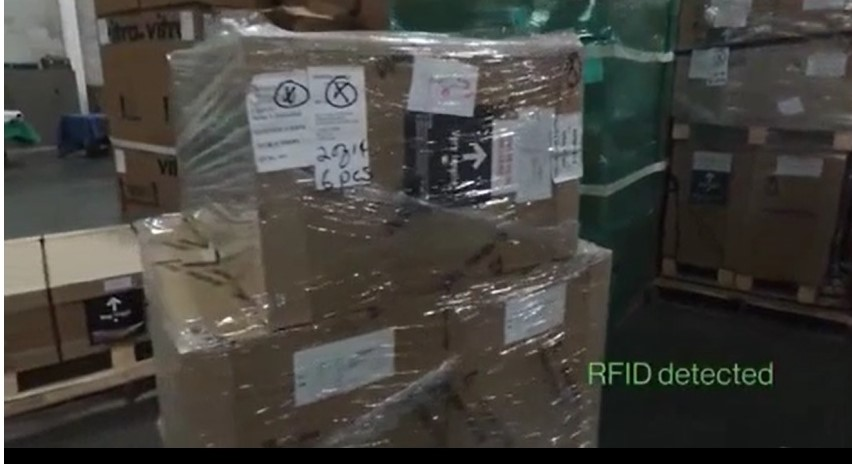
\includegraphics[width=0.33\textwidth]{imgs/MIT1.jpg}}
  \subfloat[RFID decodificado]{
   \label{f:RFID decodificado}
    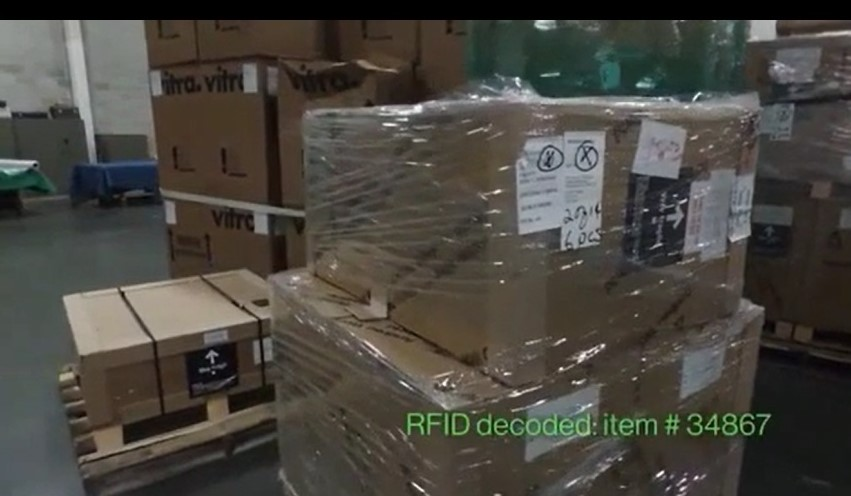
\includegraphics[width=0.33\textwidth]{imgs/MIT2.jpg}} 
  \subfloat[Item RFID localizado]{
   \newline\label{f:Item RFID localizado}
    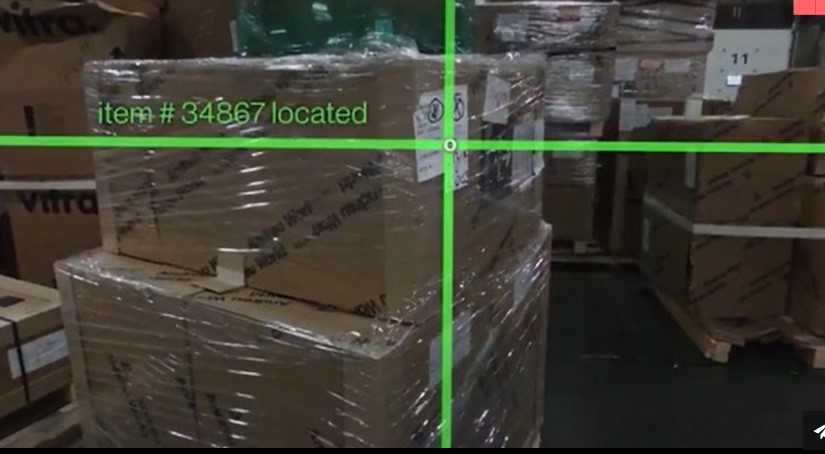
\includegraphics[width=0.33\textwidth]{imgs/MIT3.jpg}} 
 \caption{Drone detectando codigo RFID.}
 \label{f:Drone detecta codigo RFID}
\end{figure} 


\hspace{1 cm} Para el traslado de mercanc\'ias en interiores tambi\'en se ha puesto en marcha la cadena de supermercados estadounidense Walmart, cuyo objetivo es transportar productos de un lugar a otro previamente establecidos. La idea de este proyecto se debe a los grandes almacenes que tienen estos supermercados, y que cuando un cliente no encuentra el producto deseado, avisa a un empleado y \'este tiene que ir al almacen a buscarlo, perdiendo mucho tiempo entre la distancia recorrida y la b\'usqueda del producto. Lo que conseguir\'ian con esto, es que en caso de que los empleados est\'en ocupados, un cliente no tenga que estar a la espera, sino que con un dispositivo podamos pedir el producto y un drone se encargar\'a de ir a por el y traerlo al punto donde nos encontremos. Destacar que se incorporaran en las tiendas controladores a\'ereos para que los veh\'iculos sigan una trayectoria segura.  



\section{Hardware de drones}
\hspace{1 cm} Hay que destacar las partes que tiene un drone y su forma, pues es gran parte lo que lo hace tan especial, permite que tenga una gran libertad de movimientos, ya que puede moverse sin problema desde cualquier punto hacia los ejes X, Y y Z. Lo que ganamos con esto son funcionalidades como poder permitirse un aterrizaje y un despegue totalmente vertical, sin depender de un espacio en el que coger velocidad para levantar el vuelo, e igual con el aterrizaje, pudiendo el drone estando quieto en el aire bajar totalmente en vertical hasta tocar posarse sobre el suelo. Una vez en el aire pueden moverse adelante, atr\'as, izquierda, derecha, arriba, abajo y combinaciones de movimientos entre ejes, adem\'as de los giros Roll, Yaw y Pitch y sin necesidad de hacer movimientos bruscos. Sin embargo, en los anteriores UAV solo tenemos el movimiento hacia adelante, teniendo que jugar con Roll, Yaw y Pitch para poder movernos en los distintos ejes.

\begin{figure}[ht]
	\centering
		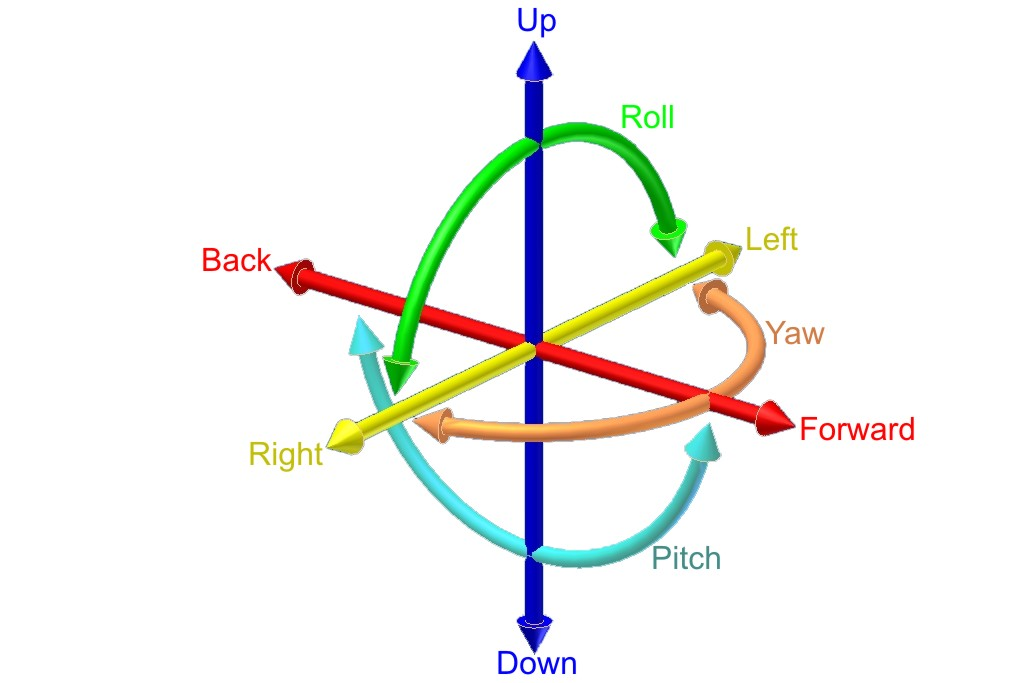
\includegraphics[width=0.7\textwidth]{imgs/ejesdrone.eps}
		\caption{Diferentes movimientos que puede realizar un drone.}
	\label{fig:ejesdrone}
\end{figure}

\hspace{1 cm} Un desglose explicando cada una de las partes ser\'ia:

\hspace{1 cm}\textbf{Marco:} Tambi\'en conocido como estructura o chasis. Es la estructura principal sobre la que se sit\'uan el resto de los elementos. Cambiar\'a su forma dependiendo del drone, variando la longitud de las patas o el n\'umero de soportes para h\'elices, por ejemplo. Puede estar hecha por diversos materiales, generalmente se trata de alg\'un tipo de pl\'astico, ya que es un material que tiene poco coste y pesa poco. Un ejemplo es el polipropileno, que es ligero y con mucha resistencia, lo que permite colocar sobre \'el la bater\'ia. Otro material que suele utilizarse es la fibra de carbono, ya que pesa poco y es muy resistente, aunque puede tener factores negativos como su conductividad. Por \'ultimo, tambi\'en nombrar la fibra de vidrio. Este material tambi\'en es muy utilizado por ser ligero, y tiene caracter\'isticas como que no es conductor de la electricidad. Es com\'un ver estructuras h\'ibridas entre distintos materiales, sobre todo juntando los dos tipos de fibra. 

\hspace{1 cm}\textbf{H\'elices:} Elemento formado por dos palas montadas de forma conc\'entrica sobre un eje, que al girar crean un par de fuerzas, permitiendo as\'i el movimiento del drone.

\hspace{1 cm}\textbf{Motores:} Son los encargados de transformar la energ\'ia que llega en movimiento sobre el eje en el que se sit\'uan las h\'elices, para as\'i permitirles a \'estas hacer su trabajo. \'Este, a su vez, tiene distintos par\'ametros que ser\'an principalmente los que permitan al drone llevar mayor velocidad: 

\begin{itemize}
\item El numero de vueltas que d\'e por minuto, lo que depender\'a de los KiloVoltios. Suele estar en torno a 800-900kV.

\item El tamaño que \'este tenga. Al mirar las especificaciones de un drone est\'a en un numero de 4 d\'igitos, en el que los dos primeros hacen referencia al tamaño del rotor y los otros dos al tamaño de la bobina. 

\item El empuje, valor que hacer referencia al peso que puede levantar el motor.

\item La corriente, se trata de la energ\'ia (amperios) que se consume cuando el motor est\'a al m\'aximo.
\end{itemize}

\hspace{1 cm}\textbf{Bater\'ia:} Encargada de proporcionar la energ\'ia suficiente para que el drone pueda realizar un vuelo, permitiendo trabajar a la placa controladora y motores. La caracter\'istica principal de las bater\'ias son los miliamperios hora, ya que es la que permitir\'a una mayor capacidad y por lo tanto que el drone tenga un mayor tiempo de vuelo. Existen bater\'ias de muy diversos tamaños, desde los 350 mah en drones de juguete a, por ejemplo, los 4500mah que tiene la bater\'ia del drone 3DR solo. Tambi\'en es importante la tasa de descarga, que es la m\'axima energ\'ia que puede entregar y el periodo de tiempo durante el que puede hacerlo. Normalmente los drones traen sistemas de alerta que avisan cuando a la bater\'ia le queda poca energ\'ia, o que cuando queda un valor menor a cierto porcentaje de carga no permite despegar el drone, evitando as\'i que se quede sin energ\'ia a mitad de un vuelo.

\hspace{1 cm}\textbf{Equipo de transmisi\'on:} Es el encargado de que se comunique el drone con una estaci\'on receptora. Puede variar en funci\'on del aparato ya que se pueden usar diferentes tecnolog\'ias, pero principalmente usa radiofrecuencia o Wifi. Existen casos, como el modelo 3DR, que combina ambas tecnolog\'ias, utilizando la radiofrecuencia para la informaci\'on del movimiento, bater\'ia y posicionamiento, y el WiFi para la transmisi\'on de im\'agenes en directo. Se pueden encontrar distintos equipos de sistemas de transmisi\'on, uno de los \'ultimos y mas destacables es Hyperion, que utiliza un sistema \'optico de comunicaciones capaz de transmitir hasta 1Gb por segundo, lo que permite la transmisi\'on de datos mediante la luz directa. Su principal caracter\'istica es que no pierde informaci\'on cuando no hay contacto directo entre las dos estaciones. La v\'ia WiFi es muy utilizado, pues permite controlar el drone desde una aplicaci\'on m\'ovil, por lo que conectando estos dos tendr\'iamos un mando que nos permite cambiar gran parte de la configuraci\'on del drone. Tambi\'en existen dispositivos que permiten el control mediante Bluetooth, pero es menos com\'un ya que tiene mayor restricci\'on de velocidad de datos y distancia. 


\hspace{1 cm}\textbf{Placa controladora:} Es el procesador del drone, el que se encarga de recoger la informaci\'on del drone y cuando le llega una orden ver que informaci\'on tiene que mandar para que \'esta se ejecute de forma correcta, as\'i como en caso de haber un problema tratar de evitarlo. Hay una gama muy amplia:
	\begin{itemize}
		\item Pixhawk: Es el m\'as utilizado debido a que trabaja con 3DRobotics y Ardupilot. Sirve para diversos dispositivos como drones, helic\'opteros y barcos. Est\'a pensado para cualquier veh\'iculo que tenga movimiento. Se trata de un proyecto hardware abierto, cuyo objetivo principal es proporcionar el hardware de autopiloto a comunidades acad\'emicas o gente que tiene esto como un hobby, teniendo as\'i un bajo costo y una alta disponibilidad. Es un piloto autom\'atico en tiempo real y muy eficiente, proporcionando un entorno de estilo POSIX. \'Este es el autopiloto est\'andar de la industria, y por lo tanto, como veremos a continuaci\'on, a partir \'el se han desarrollado diversos autopilotos con distintas mejoras. 

		\item Pixhawk2:\footnote{\url{https://pixhawk.org/}} Es una versi\'on avanzada de la placa anterior. Tiene mejoras como aislamiento de vibraciones, 3 IMUs para redundancia (3 aceler\'ometros, 3 giroscopos, 3 magnet\'ometros y 2 bar\'ometros) y sensor para controlar la temperatura. 

		\item PixRacer: Se ha desarrollado para los drones de carreras, aunque tambi\'en se utiliza en minidrones. Suele tener una mayor memoria flash.

		\item Navio2: Piloto autom\'atico diseñado de Raspberry Pi. Te permite convertir \'esta en un controlador de drone. 

		\item PXFmini: Es otro piloto autom\'atico de Raspberry Pi. \'Este tiene la electr\'onica para la mayor\'ia de los componentes que puede utilizar un drone. 

		\item FlytPOD: Es una placa Odroid XU4 SBC junto con una PixHawk. Puede volar diversos veh\'iculos a\'ereos y su principal caracter\'istica es el WiFi que tiene integrado. Existe una placa FlytPOD pro que es una versi\'on extendida de la anterior, con m\'as sensores y mayor capacidad de almacenamiento. 

		\item U-Pilot: Este hardware se caracteriza por servir para diversos veh\'iculos a\'ereos, siendo programable para realizar todas las acciones de su camino de forma autom\'atica. Su radioenlace con frecuencia en torno a 900Mhz permite controlar el dispositivo a una distancia de 100km. 
	\end{itemize}

\hspace{1 cm} Hay que destacar un elemento importante como es la c\'amara, que aunque no todos los drones la llevan s\'i es bastante com\'un. Algunos la llevan incorporada (incluso dos c\'amaras, una que apunta hacia la parte de delante y otra que apunta la parte de abajo) y otras que traen soporte para incorporar ciertas c\'amaras, normalmente consideradas c\'amaras de acci\'on, para obtener una mejor calidad. Algunos drones incorporan una Gimbal para controlar la parte hacia la que queremos que apunte la c\'amara en cada momento o utilizarlo como estabilizador, para evitar as\'i que afecten a la imagen diversos movimientos, generalmente bruscos, que pueda realizar el drone. 

\hspace{1 cm} En ocasiones, utilizado normalmente para carreras de drones, la c\'amara sirve para integrar la tecnolog\'ia FPV (First Person View), que es junto a la c\'amara, el transmisor de v\'ideo y el receptor de v\'ideo, poder ver en tiempo real las im\'agenes sobre una pantalla LCD o utilizando unas gafas de realidad virtual. En esta linea uno de los sistemas m\'as impactantes es el conjunto que se ha creado con el done \textbf{FLYBi}, estando \'este conectado a unas gafas de realidad virtual que tienen sensor de movimiento, lo que te permite sentir que eres t\'u el que vuelas y el que est\'as en el lugar del drone, y con cualquier movimiento que sientan las gafas la c\'amara del drone lo imitar\'a. En caso de que esto parezca inc\'omodo tiene un joystick con el que tambi\'en se pueden ordenar los movimientos realizar a la c\'amara. 
 

\begin{figure}[H]
 \centering
  \subfloat[Chasis]{
   \label{f:chasis}
    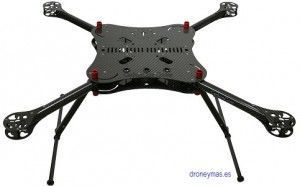
\includegraphics[width=0.2\textwidth]{imgs/chasis-drone.jpg}}
  \subfloat[H\'elices]{
   \label{f:helices}
    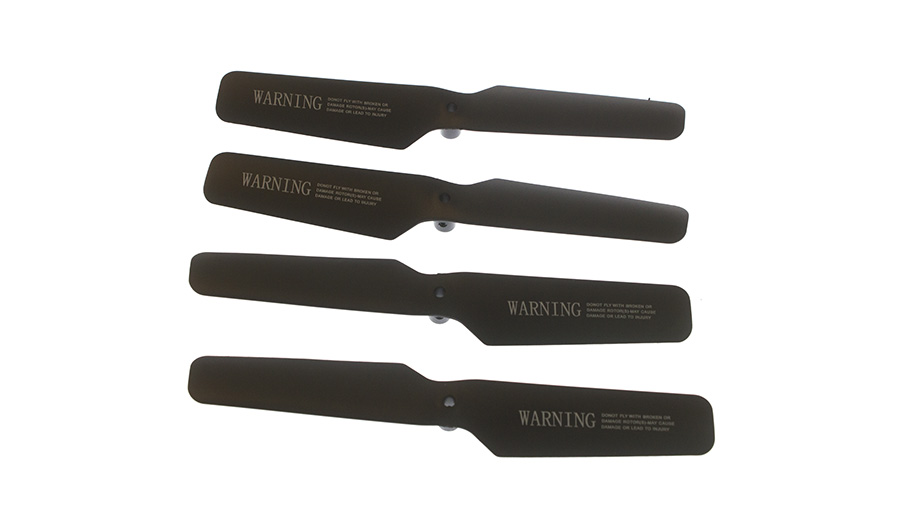
\includegraphics[width=0.2\textwidth]{imgs/helices-drone.jpg}}
  \subfloat[Motor]{
   \newline\label{f:motor}
    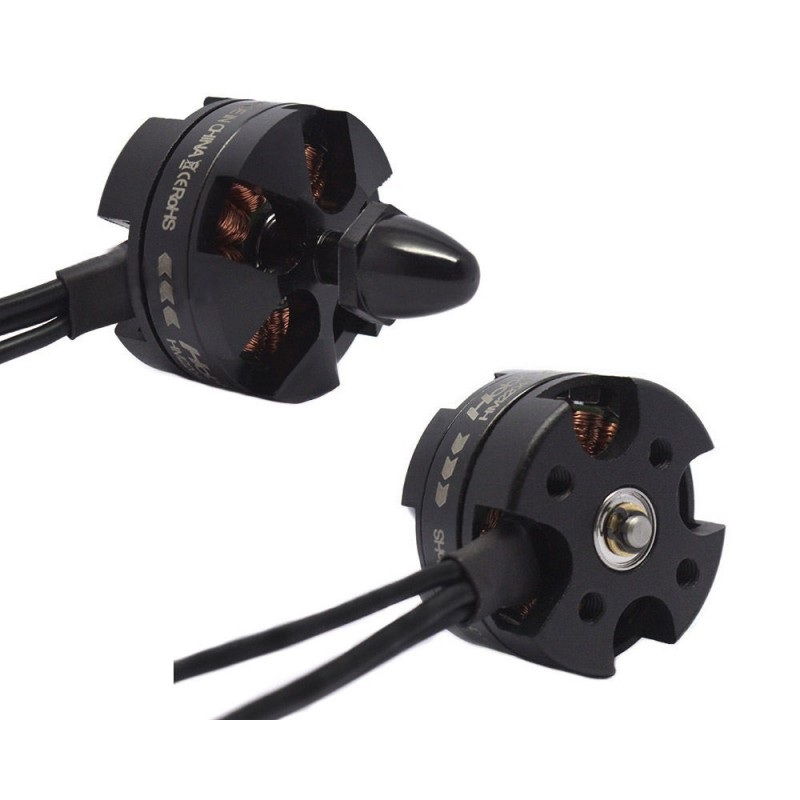
\includegraphics[width=0.2\textwidth]{imgs/motor-drone.jpg}}
	\subfloat[Placa-Madre]{
   \newline\label{f:placa-madre}
    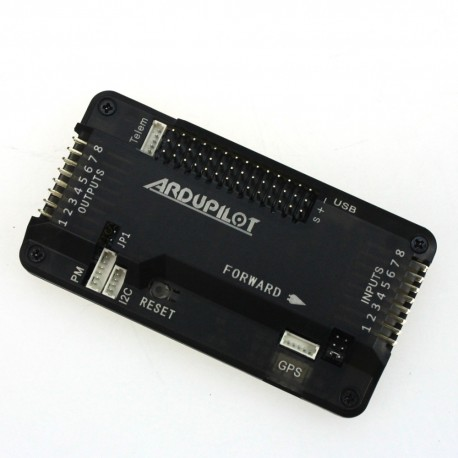
\includegraphics[width=0.2\textwidth]{imgs/placaControladora-drone.jpg}}
 \caption{Distintas partes del drone.}
 \label{f:Test 1}
\end{figure} 


\section{Software de drones}
\hspace{1 cm} El software es el conjunto de programas que permiten realizar ciertas tareas, por ejemplo al drone una navegaci\'on aut\'onoma. Dicho programa estar\'a instalado en la placa controladora, y por tanto ser\'a el que ejecute para recoger la distinta informaci\'on de los sensores, procesar la informaci\'on y enviar las \'ordenes correctas a los distintos elementos. El desarrollo de software para este tipo de robots ha evolucionado mucho en los \'ultimos años debido al uso civil que se le comienzan a dar y no tanto al desarrollo militar. Existen varios entornos software que permiten el manejo y la programaci\'on de estos robots:

	\begin{itemize}
		\item \textbf{Ardupilot:} Es un sistema OpenSource encargado de recibir la informaci\'on que se le da y de enviar las señales correspondientes a los actuadores. Se trata del software m\'as importante por lo completo que es y la confiabilidad que proporciona, debido a la gran cantidad de gente que lo utiliza (pilotos de drones profesionales y aficionados) y por el equipo de ingenieros que lo han desarrollado. Este software se caracteriza por la variedad de dispostivos que puede llegar a controlar, ya que trabaja con diversos dispositivos a\'ereos (aviones, helic\'opteros, drones, etc) y con dispositivos marinos (como son los barcos y submarinos). \'Este ha tenido un gran desarrollo debido a que es c\'odigo abierto. Hay mucha gente creando interfaces para \'el y dichos usuarios comparten sus avances con el resto. A partir de \'este han nacido controladores como Ardupilot Mega. El problema que tiene dicho software es que s\'olo permite trabajar con plataformas de los mismos creadores. Otra caracter\'istica es la facilidad con la que se le pueden añadir diferentes sensores, como pueden ser modulos GPS o c\'amaras, algo que facilita la navegaci\'on aut\'onoma. 

	\item \textbf{Megapirate-NG:} Apareci\'o como desarrollo del anterior. La funcionalidad de uno y otro es pr\'acticamente la misma, con la diferencia de que \'este permite trabajar con Hardware de otros creadores. El problema es que siempre depende de Ardupilot, por lo tanto sus funcionalidades, aunque sean m\'as c\'omodas para trabajar, puede que est\'en atrasadas.

		\item \textbf{MultiWii:} Se propuso como radiocontrol para drones. Es un sistema que fue creado por los desarrolladores y con los sensores (giroscopios y aceler\'ometros) de la Nintendo Wii. Es una plataforma basada en arduino, con el factor en contra de tener una funcionalidad bastante limitada. 
	\end{itemize}


Estos son los entornos software principales que estar\'ian sobre el veh\'iculo, pero tambi\'en est\'an los programas que se ejecutar\'ian en otros dispositivos como el ordenador o el tel\'efono m\'ovil para ver la informaci\'on que \'este nos env\'ia. Normalmente el fabricante del drone tiene ya un programa que realiza esta funci\'on. 

\hspace{1 cm} En este punto es importante el protocolo de comunicaci\'on que habr\'a para comunicar el veh\'iculo con la estaci\'on terrena. Aqu\'i hay un protocolo que destaca sobre los dem\'as, el MAVLink (Micro Air Vehicle Communication Protocol). \'Este protocolo tiene la informaci\'on contenida en ficheros .xml, lo que permite utilizarlo en diversos lenguajes de comunicaci\'on, y conlleva una mejora notable en su desarrollo. Al tener el fichero .xml los tipos de mensaje, permite con facilidad añadir nuevos tipos para asignar una tarea nueva. Otra ventaja es que hay muchos software de drones que lo soportan, como pueden ser Ardupilot, Autopilot, algunos derivados de \'estos y otros como Gentlenav o Flexipilot, y desde la estaci\'on tierra algunos como MAVProxy, Mission Planer o APM planner. 
Un problema en este protocolo es que los datos no est\'an encriptados en la comunicaci\'on, por lo que es m\'as f\'acil un ataque y que se manipulen los datos. Adem\'as detecta si se pierde alg\'un dato ya que utiliza CRC (codigo de redundancia c\'iclica para detectar cambios en los datos, este se utiliza en protocolos como TCP).
MAVLink utiliza otro software llamado MAVProxy para acceder a los datos del veh\'iculo, como la velocidad y las im\'agenes, lo que nos permitir\'a tambi\'en saber qu\'e datos mandarle para que funcione de forma correcta. 

\hspace{1 cm} A parte de todos \'estos, existen tambi\'en otras infraestructuras software como puede ser \textbf{JdeRobot}, que es la que hemos usado en este trabajo y que se describir\'a con mas detalle en el cap\'itulo 3. 


	

\section{Rob\'otica a\'erea en RoboticsLab de la URJC}
\hspace{1 cm} En un contexto mas cercano, este proyecto se inici\'o tras otros realizados anteriormente en el laboratorio de rob\'otica de la universidad. Los ejemplos mas destacables son los siguientes:


%Es importante destacar que el inicio de este proyecto se ha podido dar gracias a otros proyectos realizados en el laboratorio de la universidad, en los que se hicieron grandes avances en el \'area de la rob\'otica a\'erea y que nos han llevado a centrarnos en el caso de la situaci\'on por visi\'on mediante balizas. Algunos casos de otros trabajos son los siguientes:

\hspace{1 cm} Alberto Mart\'in \footnote{http://jderobot.org/Amartinflorido-tfm} \cite{MediaWikiAlbertoMartinFlorido} trabaj\'o en el seguimiento de objetos con un drone utilizando su c\'amara. Ten\'ia un controlador reactivo PID, y el drone ten\'ia que seguir una pelota de color rosa, consiguiendo que le siguiera en un espacio 3D, seg\'un muestra la figura \ref{f:AlbertoMartin}. El drone en caso de no encontrar la pelota rosa se quedaba parado donde estuviera. Adicionalmente en este proyecto se desarrollo el driver para el ArDrone del Parrot real, que es el mismo que hemos utilizado en este proyecto.
\begin{figure}[H]
 \centering
    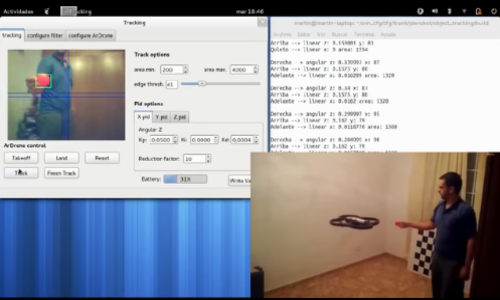
\includegraphics[width=0.4\textwidth]{imgs/AlbertoMartin1_1.png}
    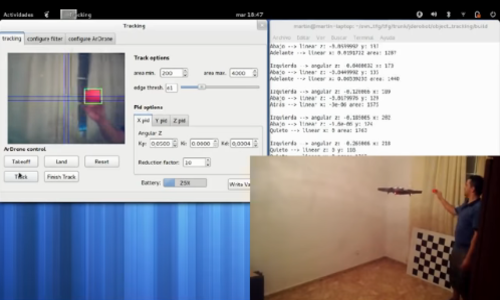
\includegraphics[width=0.4\textwidth]{imgs/AlbertoMartin2_1.png}
 \caption{TFG Alberto Mart\'in.}
 \label{f:AlbertoMartin}
\end{figure} 


\hspace{1 cm} Arturo Velez \footnote{\url{http://jderobot.org/Avelez-tfg}} \cite{MediaWikiArturoVelezDuque} trabaj\'o en un seguimiento visual pero sin filtro de color, en el cual un drone debe seguir una textura que se mueve por el suelo detectando los puntos de inter\'es. En caso de que el drone pierda la referencia de la figura en la imagen, realiza un algoritmo de b\'usqueda.
\begin{figure}[H]
 \centering
    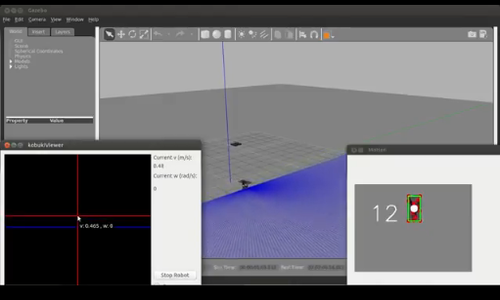
\includegraphics[width=0.4\textwidth]{imgs/ArturoVelez1_1.png}
    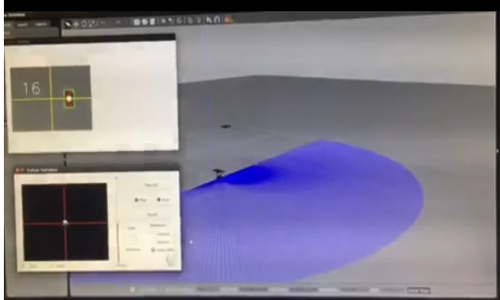
\includegraphics[width=0.4\textwidth]{imgs/ArturoVelez2_1.png}
 \caption{TFG Arturo Velez.}
 \label{f:ArturoVelez}
\end{figure} 


\hspace{1 cm} Manuel Zafra trabaj\'o \footnote{\url{http://jderobot.org/Mazafrav-pfc}} \cite{MediaWikiManuelZafraVillar} en la localizacion del drone mediante April Tags. El objetivo de \'este era recorrer aut\'onomamente una ruta tridimensional en interiores, como secuencia de puntos 3D para lo que necesitaba estar localizado. Gracias a las April Tags que detectaba el drone pod\'ia detectar el punto en un mapa 3D en el que estaba situado como se muestra en la figura \ref{f:ManuelZafra}
\begin{figure}[H]
 \centering
    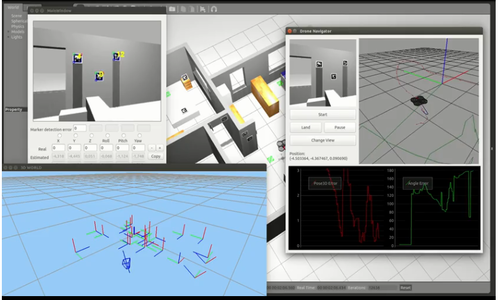
\includegraphics[width=0.4\textwidth]{imgs/ManuelZafra1_1.png}
    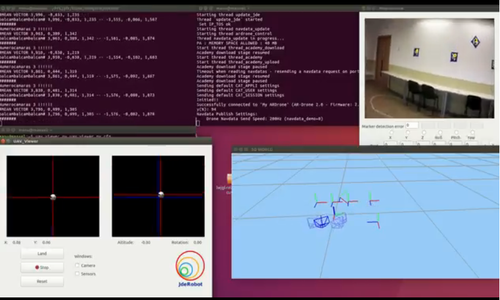
\includegraphics[width=0.4\textwidth]{imgs/ManuelZafra2_1.png}
 \caption{TFG Manuel Zafra.}
 \label{f:ManuelZafra}
\end{figure} 

\hspace{1 cm} Danuel Yag\"ue \footnote{\url{http://jderobot.org/Daniyague-pfc}} \cite{MediaWikiDanielYagueSanchez} trabaj\'o con el ArDrone sobre Gazebo, probando distintas funcionalidades y escenarios. Por un lado trabaj\'o en el driver para el cuadricoptero simulado, consiguiendo un plugin para el ArDrone que proporciona los datos de los sensores a bordo y que acepta y ejecuta ordenes como despegar, aterrizar y los distintos movimientos de vuelo. Por otro lado sobre simulador program\'o aplicaciones de control visual, haciendo que el drone siguiera una linea, una carretera o que un drone siguiera al otro, como se muestra en la figura \ref{f:DanielYague}
\begin{figure}[H]
 \centering
    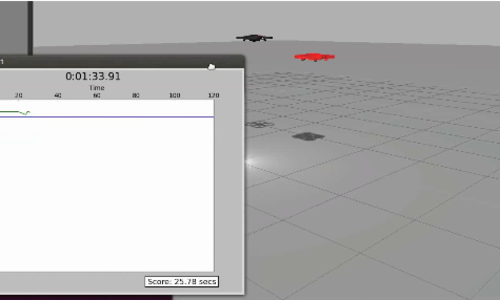
\includegraphics[width=0.4\textwidth]{imgs/DaniYague1_1.png}
    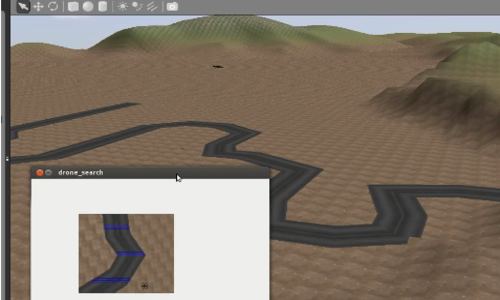
\includegraphics[width=0.4\textwidth]{imgs/DaniYague2_1.png}
 \caption{TFG Daniel Yag\"ue.}
 \label{f:DanielYague}
\end{figure} 


\hspace{1 cm} Jorge Cano \footnote{\url{http://jderobot.org/J.canoma-tfg}} \cite{MediaWikiJorgeCanoMartinez} trabaj\'o en el diseño, construcci\'on y programaci\'on de un drone real. El driver que realiz\'o para su control se basa en el protocolo MAVLink, en parte por su gran popularidad. Por una parte trabaj\'o en el diseño y construcci\'on de la plataforma hardware y por otra en el contolador software para la comunicaci\'on con el veh\'iculo. Para hacer tests de vuelo realiz\'o pruebas perceptivas y de control, con filtros de colores y un controlador PID.

\begin{figure}[H]
 \centering
    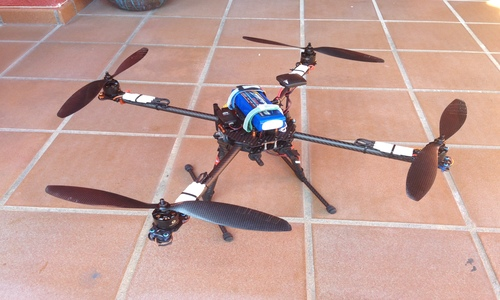
\includegraphics[width=0.3\textwidth]{imgs/JorgeCano1_1.jpg}
    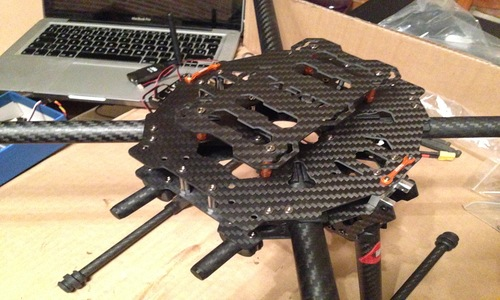
\includegraphics[width=0.3\textwidth]{imgs/JorgeCano2_1.jpg}
    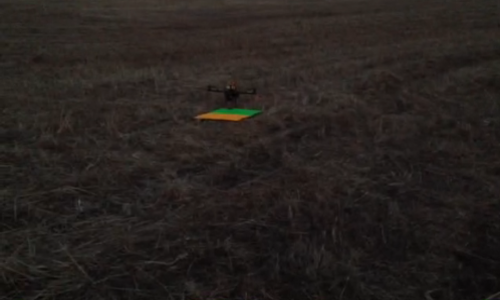
\includegraphics[width=0.3\textwidth]{imgs/JorgeCano3_1.png}
 \caption{TFG Jorge Cano.}
 \label{f:JorgeCano}
\end{figure} 

% Alberto Mart\'in trabaj\'o en la navegaci\'on visual para el seguimiento de objetos. En este proyecto el drone trabajaba en los ejes X,Y y Z. Teniendo un objeto de determinadas caracter\'isticas el drone era capaz de seguirlo, funcionando tanto en el eje vertical como en el horizontal. Tambi\'en era capaz de cambiar la orientaci\'on del drone en funci\'on de la situaci\'on del objeto. 

%\hspace{1 cm} Daniel Yag\"ue trabaj\'o en con el ArDrone sobre gazebo, probando distintas funcionalidades y distintos escenarios. En este proyecto, tambi\'en mediante control visual, realiz\'o diversas pruebas como seguir l\'ineas, seguir otro drone o seguir un recorrido mediante April Tags. 

%\hspace{1 cm} Manuel Zafra trabajo en la localizaci\'on del Drone mediante April Tags. En este proyecto el drone iba detectando las diferentes April Tags que hab\'ia situadas en los distintos lugares y gracias a ello sab\'ia la posici\'on en la que se encontraba y los movimientos a realizar.  

%\hspace{1 cm}Arturo Velez realiz\'o un proyecto en el cual el drone segu\'ia un objeto dada una textura y la autolocalizaci\'on a partir de \'esta. Si no se encontraba la textura el drone realizaba una b\'usqueda. Tambi\'en trabaj\'o con April Tags y la autolocalizaci\'on en funci\'on de lo que detectaba.

%\hspace{1 cm} Por \'ultimo nombrar el proyecto de Jorge Cano, quiz\'as es el mas distinto a los anteriores y a lo que se ha trabajado aqu\'i, ya que se centraba m\'as en el hardware del drone, especificando los distintos materiales y su configuraci\'on con el software. Destacar que tami\'en realiz\'o pruebas de vuelo para las cuales tuvo que trabajar en las partes perceptiva y de control.

\hspace{1 cm} Una vez terminada la breve introducci\'on, se va a explicar lo realizado en este proyecto. En el cap\'itulo 2 se redactan los objetivos propuestos y la metodolog\'ia seguida para llegar hasta ellos. En el cap\'itulo 3 se presenta la infraestructura utilizada y como se ha trabajado con ella. En el cap\'itulo 4 se describe el algoritmo realizado, c\'omo se ha programado y porqu\'e se han seguido unos u otros caminos. En el cap\'itulo 5 se detalla los distintos experimentos realizados y los resultados que se han obtenido. Por \'ultimo, en el cap\'itulo 6 se incluyen las conclusiones a las que se han llegado tras finalizar este proyecto.









